\chapter{Side-channel using Reorder Buffer}

% Reorder buffer is used by Out-of-Order cores for in-order retirement.
% In SMT cores, fairness policy ensures that roughly equal instructions are retired for all threads to maintain equal IPC.
% Simple implementation is to share retire pipeline width equally among threads.
% But when one thread is stalled, other thread will use full pipeline width to retire.
% IPC of other threads will see a slight increase.
% Data-dependent branch misses and cache misses can be infered from IPC information.

Reorder buffer is an important component of an Out-of-Order core utilised in the
Tomasulo algorithm. It stores the incoming order of instructions before they
are issued in an out-of-order fashion. In an SMT context, this Reorder Buffer
may either be shared among threads or statically partitioned. The commit
stage of the pipeline retires instructions from the buffer as and when they get
ready i.e. finish execution. The commit stage will have a width equal
to the pipeline width, so a 4-wide pipeline will have a commit stage which
retires 4 instructions at max in a single cycle.

This allows for a side-channel leakage to occur because a shared Reorder Buffer
and a shared commit stage will lead to interference among the two thread's IPC.
\Figref{rob_attack} shows how stalling of Thread 1 may lead to increase in IPC of Thread 2 because it can now utilise the full commit width.

\begin{figure}
    \centering
    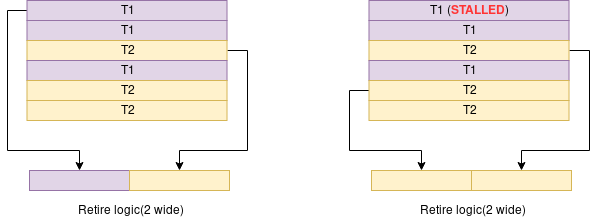
\includegraphics[width=0.8\textwidth]{rob_side_channel}
    \caption{Reorder buffer for SMT. When T1 is stalled T2 retires twice as
    many instructions.}
    \label{rob_attack}
\end{figure}

If Thread 2 can determine with reasonable accuracy when Thread 1 is stalled,
then we can infer the data being processed if those stalls are data dependent.
Data dependent stalls can include cache misses and branch mispredictions.
As we have seen in previous chapters, encryption algorithms contain such
data dependent loads and branches.
